\documentclass[12pt%
%,draft%
,xcolor=table
,aspectratio=169%
]{beamer}
%
\usepackage{fontspec}
\defaultfontfeatures{Ligatures=TeX}
%\setsansfont{Liberation Sans}
\usepackage{polyglossia}
\setdefaultlanguage{ngerman}
% Alternative template for talks of the Freie Universität Berlin.
% Created by Leonard R. König, <leonard.koenig@fu-berlin.de> following the
% guidelines on www.fu-berlin.de/cd
%
% (c) Leonard König, CC BY 4.0
%
% This template was written against UTF-8 capable LaTeX engines, specifically
% LuaLaTeX.

% Trying to get rather close to the ppt/odp template:
%  http://www.fu-berlin.de/sites/cd/downloads_container/PowerPoint_Praesentation_Anleitung.pdf

%%% font styles
\setbeamerfont{frametitle}{series=\bfseries}
\setbeamerfont{footline}{series=\bfseries}
\setbeamerfont{headline}{series=\bfseries}
\setbeamerfont{alerted text}{series=\bfseries}
%%%

% colordefs
\definecolor{fu_darkblue}{RGB}{0,51,102}
\definecolor{fu_seablue}{RGB}{0,102,204}
\definecolor{fu_lightblue}{RGB}{204,214,224}
\definecolor{fu_green}{RGB}{153,204,0}
\definecolor{fu_lightgrey}{RGB}{128,128,128}
\definecolor{fu_grey}{RGB}{95,95,95}
%
\definecolor{fu_red}{RGB}{204, 0, 0} % red text (used by \alert)
%%% end colordefs

%%% colors
\setbeamercolor*{title}{fg=fu_darkblue}
\setbeamercolor*{subtitle}{fg=fu_seablue}
\setbeamercolor*{frametitle}{fg=fu_darkblue}
\setbeamercolor*{footline}{fg=fu_grey,bg=fu_lightblue}
\setbeamercolor*{headline}{fg=fu_grey}

\setbeamercolor*{normal text}{fg=black}
\setbeamercolor*{alerted text}{fg=fu_red}
\setbeamercolor*{example text}{fg=fu_green}
\setbeamercolor*{structure}{fg=fu_darkblue}

\setbeamercolor*{block title}{fg=white,bg=black!50}
\setbeamercolor*{block title alerted}{fg=white,bg=black!50}
\setbeamercolor*{block title example}{fg=white,bg=black!50}

\setbeamercolor*{block body}{bg=black!10}
\setbeamercolor*{block body alerted}{bg=black!10}
\setbeamercolor*{block body example}{bg=black!10}

\setbeamercolor{bibliography entry author}{fg=fu_darkblue}

\setbeamercolor{item}{fg=fu_darkblue}
\setbeamercolor{navigation symbols}{fg=fu_lightgrey,bg=fu_grey}
%%% end colors

%%% title page
% Display logo (if exists) and right next to it, put our title + subtitle
\defbeamertemplate*{title page}{fu_titlepage}
{%
	\hskip .3\textheight
	\begin{minipage}[.4\textheight]{\textwidth}
		\begin{minipage}[.4\textheight]{0.25\textwidth}
			\inserttitlegraphic
		\end{minipage}%
		\begin{minipage}[.4\textheight]{0.75\textwidth}
			\begin{beamercolorbox}{title}
				\usebeamerfont{title}\inserttitle\par%
			\end{beamercolorbox}
			\vfill
			\ifx\insertsubtitle
				\@empty%
			\else
				\begin{beamercolorbox}{subtitle}
					\usebeamerfont{subtitle}\insertsubtitle\par
				\end{beamercolorbox}
			\fi
		\end{minipage}
	\end{minipage}%
	\hskip .3\textheight
}
%%% end title page

%%% headline
% display title, author and institute on the left;
% logo on the right.
\newcommand{\headlinetext}
{%
	\inserttitle\\[0.3em]%
	\insertauthor, %
	\insertshortinstitute
}
\newlength{\headlinewidth}
\setlength{\headlinewidth}{\paperwidth}
\addtolength{\headlinewidth}{-2\marginparsep}
\setbeamertemplate{headline}
{%
	\begin{beamercolorbox}[wd=\paperwidth]{headline}%
		\vskip5pt
		{\hspace*{\marginparsep}}%
		\parbox{.5\headlinewidth}
		{%
			\usebeamertemplate{title in head/foot}%
			\headlinetext%
		}%
		\begin{minipage}{.5\headlinewidth}%
			\hfill\usebeamertemplate*{logo}
		\end{minipage}%
		{\hspace*{\marginparsep}}%
	\end{beamercolorbox}%
}
%%% end headline

%%% footline
% title + date on the left, frame number on the right
\newcommand{\footlinetext}
{%
	\usebeamerfont{shorttitle}\insertshorttitle, %
	\usebeamerfont{shortdate}\insertshortdate
}
\setbeamertemplate{footline}
{%
	\begin{beamercolorbox}{footline}
		\vskip2pt
		\hspace{\marginparsep}%
		\footlinetext\hfill%
		\insertframenumber%
		\hspace{\marginparsep}
		\vskip2pt
	\end{beamercolorbox}%
}
%%% end footline

% don't use default templates for sidebars
\setbeamertemplate{sidebar right}{}
\setbeamertemplate{sidebar left}{}
\setbeamertemplate{title page}[fu_titlepage]
\usepackage{amsmath}
\usepackage{amsfonts}
\usepackage{amssymb}
\usepackage{graphicx}
\usepackage{algorithm}
\usepackage[noend]{algpseudocode}
%\usepackage{algorithmic}
\usepackage{tikz}
\usetikzlibrary{arrows,shapes,automata,petri,positioning,calc}
\usepackage{graphicx}
\usepackage{subfig}
\usepackage{pgfplots}
\usepackage{ stmaryrd }
\usepackage[normalem]{ulem}
\usepackage{circuitikz}
\usepackage{csquotes}
\usepackage{listings}


\setbeamercolor{block title}{use=structure,fg=white,bg=structure.fg!75!black}
\setbeamercolor{block body}{parent=normal text,use=block title,bg=block title.bg!10!bg}


\usepackage{expl3}

\ExplSyntaxOn
\cs_new:Npn \displayasdecimal#1 {(#1) \sb {10}}
\cs_new:Npn \displayasoctal #1 {(\int_to_oct:n{#1}) \sb 8}
\cs_new:Npn \displayasbinary #1 {(\int_to_bin:n{#1}) \sb 2}
\ExplSyntaxOff

\newcounter{divline}
\def\rlwd{.5pt} \def\rlht{\dimexpr\dp\strutbox+\ht\strutbox} \def\rldp{.75ex}
\newcommand\mydiv[3][\relax]{%
  \ifx\relax#1\stepcounter{divline}\else\setcounter{divline}{#1}\fi%
  \mbox{}\hspace{\thedivline\dimexpr1ex}#2~\setbox0=\hbox{~$#3$}%
  \dumbstackengine{-\rlwd}{\rule[-\rldp]{\rlwd}{\rlht}~#3}{\rule{\dimexpr4pt+\wd0}{\rlwd}}%
}
\def\remainder#1{\stepcounter{divline}%
  \mbox{}\hspace{\dimexpr1ex+\thedivline\dimexpr1ex}~#1\setcounter{divline}{0}}
\makeatletter
\global\newlength\@stackedboxwidth
\newlength\@boxshift
\newsavebox\@addedbox
\newsavebox\@anchorbox
\newcommand*\dumbstackengine[3]{%
    \sbox{\@anchorbox}{$#2$}%
    \sbox{\@addedbox}{$#3$}%
    \setlength{\@stackedboxwidth}{\wd\@anchorbox}%
      \ifdim\wd\@addedbox>\@stackedboxwidth%
        \setlength{\@stackedboxwidth}{\wd\@addedbox}%
      \fi%
        \setlength{\@boxshift}{\dimexpr-\dp\@anchorbox -\ht\@addedbox -#1}%
        \usebox{\@anchorbox}%
        \hspace{-\wd\@anchorbox}%
        \raisebox{\@boxshift}{\usebox{\@addedbox}}%
        \hspace{-\wd\@addedbox}%
        \hspace{\@stackedboxwidth}%
}

\newcommand\decbin[9]{%
\par\smallskip
\makebox[3cm][r]{$#1$\ }\fbox{#2}\,\fbox{#3}\,\fbox{#4}\,\fbox{#5}\,\fbox{#6}\,\fbox{#7}\,\fbox{#8}\,\fbox{#9}\par}


\def\unsignedbytecalc#1{%
\par\smallskip
\noindent$#1_{10}$\par
\smallskip
\gdef\result{}%
$\left.\begin{array}{r@{\quad}|c}\udbc{#1}\end{array}\right\}\result$\par}

\def\udbc#1{%
\ifnum#1=\z@
\expandafter\@gobble
\else
\expandafter\@firstofone
\fi
{2)\!\underline{\,#1}&\edef\r{\ifodd#1 1\else 0\fi}\r\xdef\result{\r\result}\\
\expandafter\udbc\expandafter{\the\numexpr(\ifodd#1 #1-1\else#1\fi)/2\relax}%
}}

\lstdefinestyle{Bash}{
  language=bash,
  showstringspaces=false,
  basicstyle=\small\sffamily,
  numbers=left,
  numberstyle=\tiny,
  numbersep=5pt,
  frame=trlb,
  columns=fullflexible,
  backgroundcolor=\color{gray!20},
  linewidth=0.9\linewidth,
  %xleftmargin=0.5\linewidth
  upquote=true,
  columns=fullflexible,
  literate={*}{{\char42}}1
         {-}{{\char45}}1
}

\lstdefinelanguage
   [x86]{Assembler}
   [x86masm]{Assembler} % based on the "x86masm" dialect
   % with these extra keywords:
   {morekeywords={CDQE,CQO,CMPSQ,CMPXCHG16B,JRCXZ,LODSQ,MOVSXD, %
                  POPFQ,PUSHFQ,SCASQ,STOSQ,IRETQ,RDTSCP,SWAPGS, %
                  eax,edx,ecx,ebx,esi,edi,esp,ebp, %
                  e8,e8d,e8w,e8b,e9,e9d,e9w,e9b, %
                  e10,e10d,e10w,e10b,e11,e11d,e11w,e11b, %
                  e12,e12d,e12w,e12b,e13,e13d,e13w,e13b, %
                  e14,e14d,e14w,e14b,e15,e15d,e15w,e15b}} %

\lstset{language=[x86]Assembler}


\lstset{language=C,
	basicstyle=\ttfamily,
   	keywordstyle=\color{blue}\ttfamily,
    stringstyle=\color{red}\ttfamily,
    commentstyle=\color{cyan}\ttfamily,
    morecomment=[l][\color{magenta}]{\#}
    showstringspaces=false,
  	basicstyle=\small\sffamily,
  	numbers=left,
  	numberstyle=\tiny,
  	numbersep=5pt,
  	frame=trlb,
  	upquote=true,
  	columns=fullflexible,
  	backgroundcolor=\color{gray!20},
  	%linewidth=0.9\linewidth,
  	literate=*{*}{\normalfont{*}}1,
}



\author{Benjamin Tröster}
\title[]{Logische Schaltungen \& PLAs }
%\subtitle[Addition \& Subtraktion]{Addition \& Subtraktion}
%\pgfdeclareimage{titlegraphic}{../res/dwarf_logo2.png}
%\titlegraphic{\pgfuseimage{titlegraphic}}
%\date{}
%\subject{}
%
% FU settings
\institute[HTW Berlin]{Hochschule für Technik und Wirtschaft Berlin}
%\pgfdeclareimage[height=0.9cm]{logo}{../res/dwarf_logo}
%\logo{\pgfuseimage{logo}}
%
\usepackage[
backend=biber,
citestyle=alphabetic,bibstyle=authoryear
]{biblatex}
\addbibresource{sources.bib}


\begin{document}

\begin{frame}
\titlepage
\end{frame}

\begin{frame}{Fahrplan}
\tableofcontents[hideothersubsections]
\end{frame}

\section{Recap: Darstellung Logikgatter}
\begin{frame}{Recap: Darstellung Logikgatter}
\begin{figure}
\center
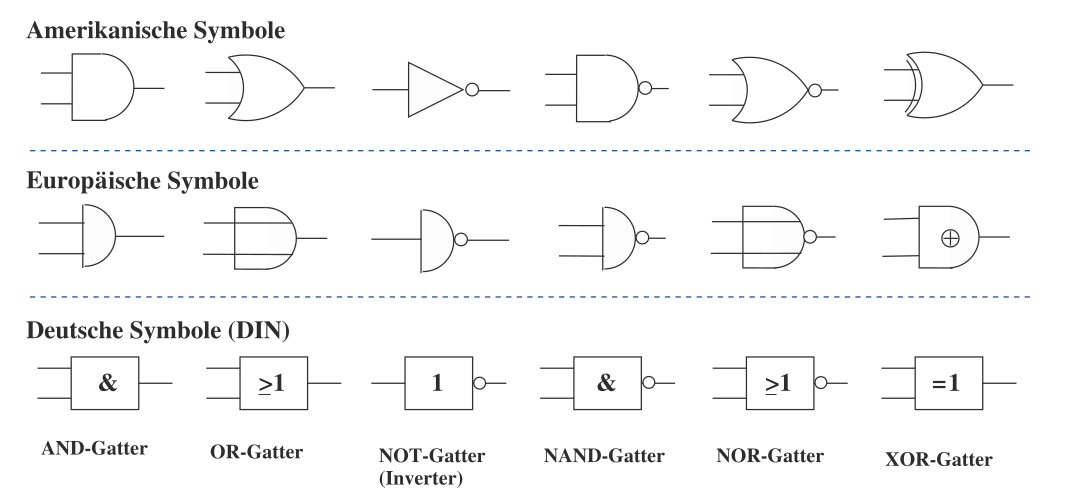
\includegraphics[scale=0.35]{pictures/logikgatter}
\caption{Übernommen aus: \cite{hoffmann2020grundlagen}}
\end{figure}
\end{frame}

\section{Logische Bausteine}
\subsection{Decoder}


\begin{frame}{Decoder}
\begin{columns}[T] % align columns
\begin{column}{.68\textwidth}
\begin{itemize}
	\item Decoder hat $n$ Eingänge und $2^n$ Ausgänge (bzw. $\leq 2^n$ Ausgänge)
	\item Für jede Eingabekombination genau einen Ausgang der 1 ergibt
	\item Alle anderen Ausgänge sind 0
	\begin{itemize}
		\item Wir codieren \enquote{Pattern} von Eingangsbits auf Ausgabebits
	\end{itemize}
	\item Beispiel: $3-to-8$-Decoder
	\begin{itemize}
		\item Ausgang $y_i$ auf $1$, alle anderen Ausgänge 0
	\item Welcher Ausgang $y_i$ auf 1 gesetzt wird, entscheiden die Eingänge $a,b,c$
	\item Eingänge $a, b$ und $c$ stellen entsprechende Dualzahl dar
	\end{itemize}
	\item Nutzung z.B. ROMs
\end{itemize}
\end{column}%
\hfill%
\begin{column}{.48\textwidth}
\centering
\vspace*{-1.7cm}
\begin{figure}
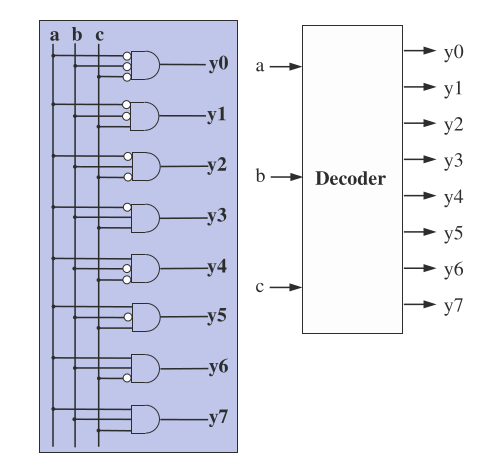
\includegraphics[scale=0.3]{pictures/decoder1}\\
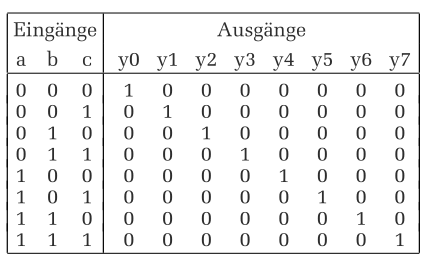
\includegraphics[scale=0.3]{pictures/decoder2}
\caption{3-to-8 Decoder Schaltung \& Wahrheitstabelle.}
\end{figure}
\end{column}%
\end{columns}
\end{frame}

\begin{frame}[fragile]{3-to-8-Decoder Beispiel in C}
\begin{lstlisting}[language=C]
int main(void) {
   int  a, b, c;
   printf("Enter encoded binary number: ");
   a = getchar() - '0';
   b = getchar() - '0';
   c = getchar() - '0';
   if (!a && !b && !c) printf("---> y0\n");
   if (!a && !b &&  c) printf("---> y1\n");
   if (!a &&  b && !c) printf("---> y2\n");
   if (!a &&  b &&  c) printf("---> y3\n");
   if ( a && !b && !c) printf("---> y4\n");
   if ( a && !b &&  c) printf("---> y5\n");
   if ( a &&  b && !c) printf("---> y6\n");
   if ( a &&  b &&  c) printf("---> y7\n");
   return 0;
}
\end{lstlisting}
\end{frame}

\subsection{Encoder}
\begin{frame}{Encoder}
\begin{columns}[T] % align columns
\begin{column}{.58\textwidth}
\begin{itemize}
	\item Analog: Encoder inverse Funktion zum Decoder
	\item Encoder hat $2^n$ Eingänge, von denen genau einer wahr sein sollte
	\item Ausgabe von $n$ Bits
	\item Beispiel: $8-to-3$-Encoder
	\begin{itemize}
		\item Eingänge $x_0 ,x_1 , \ldots x_7$ auf Codierung in Dual an den Ausägangen $d_2 , d_1 , d_0$
	\end{itemize}
\end{itemize}
\end{column}%
\hfill%
\begin{column}{.48\textwidth}
\centering
\vspace*{-1.7cm}
\begin{figure}
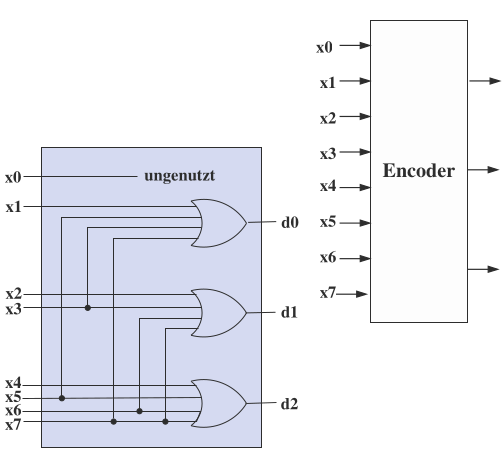
\includegraphics[scale=0.3]{pictures/encoder1}\\
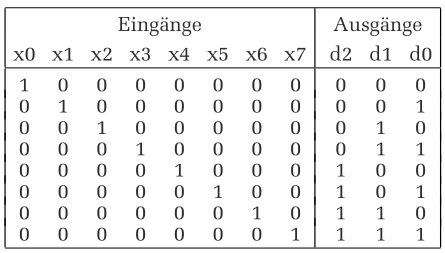
\includegraphics[scale=0.3]{pictures/encoder2}
\caption{8-to-3 Enocer Schaltung \& Wahrheitstabelle.}
\end{figure}
\end{column}%
\end{columns}
\end{frame}

\begin{frame}[fragile]{8-to-3-Encoder Beispiel in C}
\begin{lstlisting}[language=C]
int main(void) {
   int  x0, x1, x2, x3, x4, x5, x6, x7, d0=0, d1=0, d2=0;
   printf("Enter8 Bit Binary Number: ");
   x0 = getchar() - '0';
   x1 = getchar() - '0';
   x2 = getchar() - '0';
   x3 = getchar() - '0';
   x4 = getchar() - '0';
   x5 = getchar() - '0';
   x6 = getchar() - '0';
   x7 = getchar() - '0';
   d0 = x1 || x3 || x5 || x7;
   d1 = x2 || x3 || x6 || x7;
   d2 = x4 || x5 || x6 || x7;
   printf("---> %d%d%d (d2, d1, d0)\n", d2, d1, d0);
   return 0;
}
\end{lstlisting}
\end{frame}

\subsection{Multiplexer}
\begin{frame}{Multiplexer (Selektor)}
\begin{columns}[T] % align columns
\begin{column}{.58\textwidth}
\begin{itemize}
	\item Multiplexer werden oft auch als Selektoren bezeichnet, da sie unter den Eingangssignalen eines auswählen
	\item Mulitplexer führt Datenpfade zusammen
	\item Multiplexer: Mehrere Eingänge und einen Ausgang
	\begin{itemize}
		\item Wobei dieser einem der Eingänge entspricht, der durch eine Steuerung ausgewählt wird
	\end{itemize}
\end{itemize}
\end{column}%
\hfill%
\begin{column}{.48\textwidth}
\centering
\vspace*{-1.7cm}
\begin{figure}
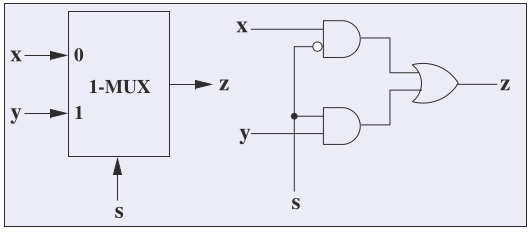
\includegraphics[scale=0.35]{pictures/mux1}\\
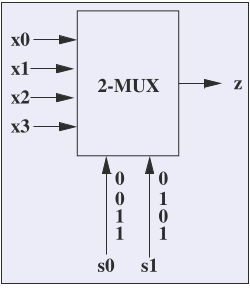
\includegraphics[scale=0.35]{pictures/mux2}
\caption{Multiplexer mit zugehöriger Schaltung und ein 2-Multiplexer.}
\end{figure}
\end{column}%
\end{columns}
\end{frame}

\begin{frame}{1-Multiplexers}
\begin{columns}[T] % align columns
\begin{column}{.68\textwidth}
\begin{itemize}
	\item 1-Multiplexers als boolesche Funktion: $z = \overline{s}x \lor sy$
	\item Was folgender Tabelle entspricht
	\item Multiplexer: Mehrere Eingänge und einen Ausgang
\begin{table}[]
\begin{tabular}{|c|c|c|}
\hline
 \textbf{$s$}& \textbf{$\overline{s}x$}  & \textbf{$sy$}  \\ \hline
0 & x & 0  \\ \hline
1 & 0  & y \\ \hline
\end{tabular}
\end{table}
	\item Bei $s=0$ wird also $x$ weitergeleitet 
	\item Bei $s=1$ wird $y$ zum Ausgang weitergeleitet.
\end{itemize}
\end{column}%
\hfill%
\begin{column}{.48\textwidth}
\centering
%\vspace*{-1.7cm}
\begin{figure}
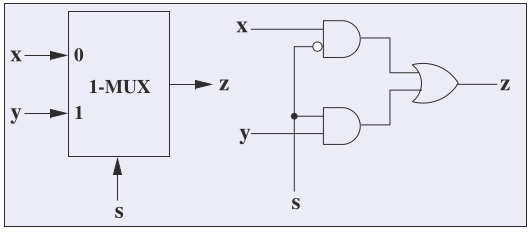
\includegraphics[scale=0.32]{pictures/mux1}
\caption{Multiplexer mit zugehöriger Schaltung.}
\end{figure}
\end{column}%
\end{columns}
\end{frame}

\begin{frame}{2-Multiplexers}
\begin{columns}[T] % align columns
\begin{column}{.68\textwidth}
\begin{itemize}
	\item Beim 2-Multiplexer sind zwei Steuereingänge vorhanden, also vier Wahlmöglichkeiten
	\item Es ergeben sich folgenden Auswahlmöglichkeiten:
\begin{table}[]
\begin{tabular}{|c|c|c|}
\hline
 \textbf{$s:0$}& \textbf{$s_1$}  & \textbf{$z$ Ausgang}  \\ \hline
0 & 0 & $x_0$  \\ \hline
0 & 1  & $x_1$ \\ \hline
1 & 0  & $x_2$ \\ \hline
1 & 1  & $x_3$ \\ \hline
\end{tabular}
\end{table}
	\item Aus dieser Tabelle lässt sich dann die folgende Schaltfunktion herleiten:
	$$ z = s_0 s_1 x_0 \lor s_0 s_1 x_1 \lor s_0 s_1 x_2 \lor s_0 s_1 x_3 $$
\end{itemize}
\end{column}%
\hfill%
\begin{column}{.48\textwidth}
\centering
%\vspace*{-1.7cm}
\begin{figure}
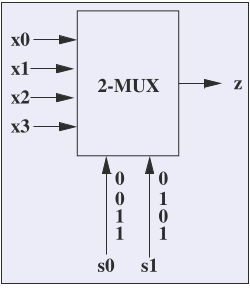
\includegraphics[scale=0.32]{pictures/mux2}
\caption{Multiplexer mit zugehöriger Schaltung und ein 2-Multiplexer.}
\end{figure}
\end{column}%
\end{columns}
\end{frame}

\begin{frame}{2-Multiplexer-Realisierung: Buttom-Up}
\begin{columns}[T] % align columns
\begin{column}{.68\textwidth}
\begin{itemize}
	\item Schaltfunktion: $z = s_0 s_1 x_0 \lor s_0 s_1 x_1 \lor s_0 s_1 x_2 \lor s_0 s_1 x_3$ bezeichnet als Buttom-Up
\end{itemize}
\end{column}%
\hfill%
\begin{column}{.48\textwidth}
\centering
%\vspace*{-1.7cm}
\begin{figure}
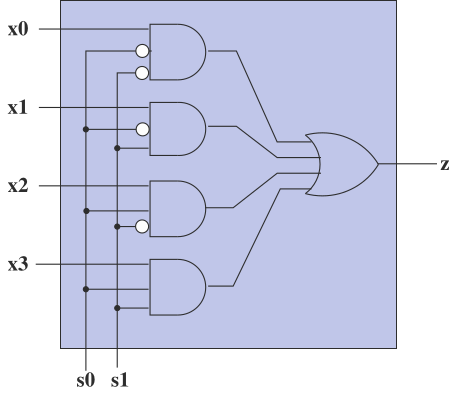
\includegraphics[scale=0.32]{pictures/mux2_bu}
\caption{Realisierung eines Buttom-Up 2-Multiplexer.}
\end{figure}
\end{column}%
\end{columns}
\end{frame}

\begin{frame}{2-Multiplexer-Realisierung: Top-Down}
\begin{columns}[T] % align columns
\begin{column}{.68\textwidth}
\begin{itemize}
	\item Top-Down-Ansatz mithilfe von 1-Multiplexern
	\item Folgendes gilt:
	\begin{enumerate}
		\item Ausgang von $1-MUX_z : z = s_0 a + s_0 b$
		\item Ausgang von $1-MUX_a : a = s_1 x_0 + s_1 x_1$
		\item Ausgang von $1-MUX_b : b = s_1 x2 + s1 x3$
	\end{enumerate}
	\item Einsetzen von $2,3$ in $1$ ergibt: $z = s_0 s_1 x_0 \lor s_0 s_1 x_1 \lor s_0 s_1 x_2 \lor s_0 s_1 x_3$
	\item Anmerkung: Top-Down braucht mehr Gatter (Preis), mehr Platz und langsamer also Button-Up
\end{itemize}
\end{column}%
\hfill%
\begin{column}{.48\textwidth}
\centering
%\vspace*{-1.7cm}
\begin{figure}
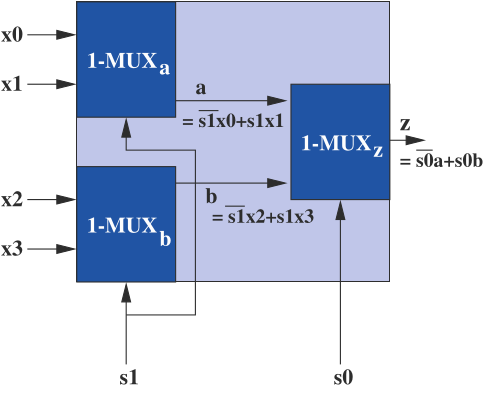
\includegraphics[scale=0.32]{pictures/mux2_td}
\caption{Realisierung eines Top-Down 2-Multiplexer.}
\end{figure}
\end{column}%
\end{columns}
\end{frame}

\begin{frame}{$n$-Multiplexer}
\begin{columns}[T] % align columns
\begin{column}{.6\textwidth}
\begin{itemize}
	\item Multiplexer mit beliebigen Anzahl von Eingaben realisierbar
	\item $n$ Eingabesignalen werden $log 2 n$ Selektoreingabe benötigt
	\item Dreiteiliger Aufbau:
	\begin{enumerate}
		\item Decoder: aus $log 2 n$ Selektoreingaben $n$ Signale erzeugt, die jeweils einen anderen Eingabewert auswählen,
		\item $n$ AND-Gattern: Kombination jeweils eines Signals des Decoder mit einem Eingabesignal 
		\item OR-Gatter: $n$ Eingängen (bzw. $n-1$ hintereinander geschaltete OR- Gatter zwei Eingängen), das die Ausgaben der AND-Gatter verknüpft.
	\end{enumerate}
\end{itemize}
\end{column}%
\hfill%
\begin{column}{.48\textwidth}
\centering
%\vspace*{-1.7cm}
\begin{figure}
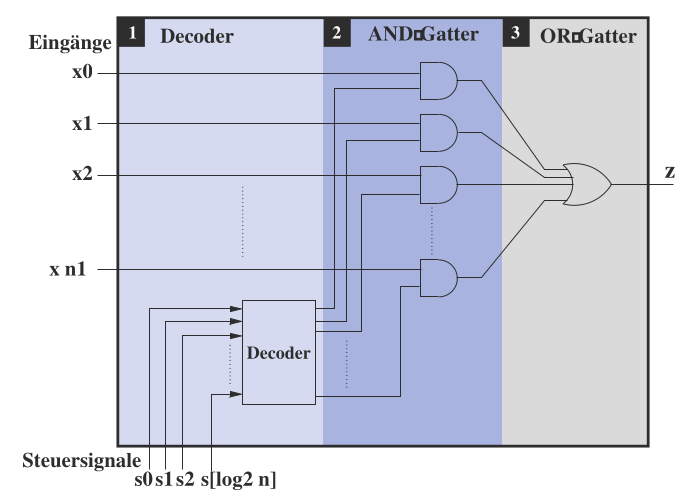
\includegraphics[scale=0.3]{pictures/nmux}
\caption{Beispiel für einen $n$-Multiplexer.}
\end{figure}
\end{column}%
\end{columns}
\end{frame}

\subsection{Demultiplexer}
\begin{frame}{Demultiplexer}
	\begin{itemize}
		\item Während für einen Multiplexer Folgendes gilt:
		\begin{itemize}
			\item $2^d$ Eingänge $(x_0 , x_1 , ..., x_{2^d} - 1$)
			\item $d$ Steuersignale $(s_0 , s_1 , ..., s_{d-1} )$ und
			\item ein Ausgang $z$ mit $z = \sum_{i=0}^{2^d-1} x_i \cdot s_0 s_1 \ldots d_{d-1}$
		\end{itemize}
		\item gilt für einen Demultiplexer Folgendes:
		\begin{itemize}
			\item ein Dateneingang $x$,
			\item $d$ Steuersignale $(s_0 , s_1 , ..., s_{d-1} )$ und
			\item $2^d$ Ausgänge $(z_0 , z_1 , ..., z_{2^d} -1 )$ mit $z_i = x \cdot s_0 s_1 ...s_{d-1}$
		\end{itemize}
		\item Demultiplexer: Steuersignale legen fest auf welchen Ausgang das Eingangssignal gelegt wird
	\end{itemize}
\end{frame}

\begin{frame}{Demultiplexer}
\begin{columns}[T] % align columns
\begin{column}{.6\textwidth}
\begin{itemize}
		\item Während für einen Multiplexer Folgendes gilt:
		\begin{itemize}
			\item $2^d$ Eingänge $(x_0 , x_1 , ..., x_{2^d} - 1$)
			\item $d$ Steuersignale $(s_0 , s_1 , ..., s_{d-1} )$ und
			\item ein Ausgang $z$ mit $z = \sum_{i=0}^{2^d-1} x_i \cdot s_0 s_1 \ldots d_{d-1}$
		\end{itemize}
		\item gilt für einen Demultiplexer Folgendes:
		\begin{itemize}
			\item ein Dateneingang $x$,
			\item $d$ Steuersignale $(s_0 , s_1 , ..., s_{d-1} )$ und
			\item $2^d$ Ausgänge $(z_0 , z_1 , ..., z_{2^d} -1 )$ mit $z_i = x \cdot s_0 s_1 ...s_{d-1}$
		\end{itemize}
		\item Demultiplexer: Steuersignale legen fest auf welchen Ausgang das Eingangssignal gelegt wird
	\end{itemize}
\end{column}%
\hfill%
\begin{column}{.48\textwidth}
\centering
%\vspace*{-1.7cm}
\begin{figure}
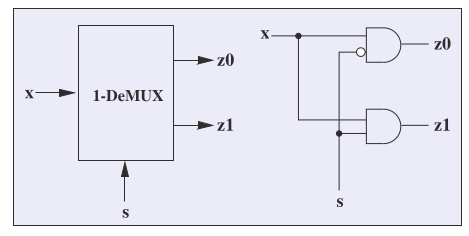
\includegraphics[scale=0.3]{pictures/demux1}\\
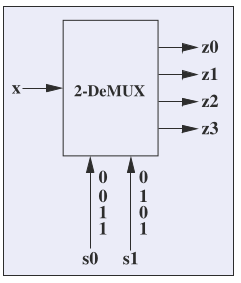
\includegraphics[scale=0.3]{pictures/demux2}
\caption{1-Demultiplexer mit zugehöriger Schaltung und ein 2-Demultiplexer}
\end{figure}
\end{column}%
\end{columns}
\end{frame}


\begin{frame}{1-Demultiplexer}
\begin{columns}[T] % align columns
\begin{column}{.6\textwidth}
\begin{itemize}
		\item $x$ steht dabei für den Eingabewert und $s$ für einen Selektor -- d.h. einen Steuerwert (control value)
		\item Steuerwert bestimmt, zu welchem der Ausgabewerte der Eingabewert weitergeleitet wird
		\item Booleschen Funktionen: $z_0 = xs$ und $z_1 = xs$
		\item Entspricht folgender Wahrheitstabelle:
		\begin{table}[]
\begin{tabular}{|c|c|cc|}
\hline
 \textbf{$s$}& \textbf{$x$}  & \textbf{Auswahl} & \textbf{Schaltfunktion} \\ \hline
0 & x & $z_0$ & $z_0 = x\overline{s}$  \\ \hline
1 & x  & $z_1$ &  $z_1 = xs$ \\ \hline
\end{tabular}
\end{table}
	\end{itemize}
\end{column}%
\hfill%
\begin{column}{.48\textwidth}
\centering
%\vspace*{-1.7cm}
\begin{figure}
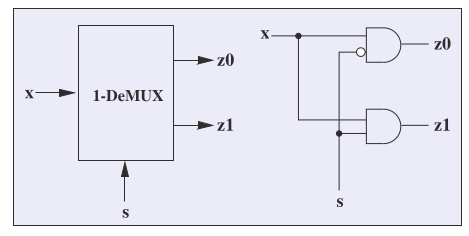
\includegraphics[scale=0.3]{pictures/demux1}\
\caption{1-Demultiplexer mit zugehöriger Schaltung.}
\end{figure}
\end{column}%
\end{columns}
\end{frame}

\begin{frame}{2-Demultiplexer}
\begin{columns}[T] % align columns
\begin{column}{.6\textwidth}
\begin{itemize}
		\item 2-Demultiplexer sind zwei Steuereingänge vorhanden $\to$ vier der Ausgabesignale auszuwählen
		\item Es ergeben sich
		\item Entspricht folgender Wahrheitstabelle:
		\begin{table}[]
\begin{tabular}{|c|c|cc|}
\hline
 \textbf{$s_0$}& \textbf{$s_1$}  & \textbf{Auswahl} & \textbf{Schaltfunktion} \\ \hline
0 & 0 & $z_0$ & $z_0 = x\overline{s_0} \overline{s_1}$  \\ \hline
0 & 1  & $z_1$ &  $z_1 = x\overline{s_0}s_1$ \\ \hline
1 & 0  & $z_2$ &  $z_2 = xs_0 \overline{s_1}$ \\ \hline
1 & 1  & $z_2$ &  $z_2 = xs_0 s_1$ \\ \hline
\end{tabular}
\end{table}
	\end{itemize}
\end{column}%
\hfill%
\begin{column}{.48\textwidth}
\centering
%\vspace*{-1.7cm}
\begin{figure}
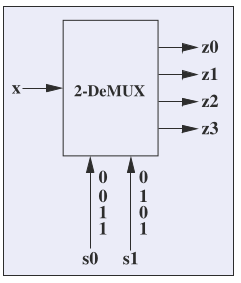
\includegraphics[scale=0.3]{pictures/demux2}\
\caption{1-Demultiplexer mit zugehöriger Schaltung.}
\end{figure}
\end{column}%
\end{columns}
\end{frame}

\begin{frame}{2-Demultiplexer-Realisierung: Buttom-Up}
\begin{columns}[T] % align columns
\begin{column}{.6\textwidth}
\begin{itemize}
		\item Direkte Realisierung als Schaltung $z_0, z_1, z_2, z_3$ in parallel
	\end{itemize}
\end{column}%
\hfill%
\begin{column}{.48\textwidth}
\centering
%\vspace*{-1.7cm}
\begin{figure}
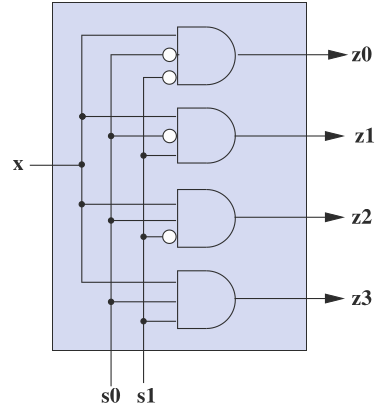
\includegraphics[scale=0.3]{pictures/2demux_bu}\
\caption{1-Demultiplexer mit zugehöriger Schaltung.}
\end{figure}
\end{column}%
\end{columns}
\end{frame}


\begin{frame}{2-Demultiplexer-Realisierung: Top-Down}
\begin{columns}[T] % align columns
\begin{column}{.6\textwidth}
\begin{itemize}
		\item Realisierung in Top-Down unter Verwendung von 1-Demultiplexern
		\item Folgende Gleichungen gelten:
		\begin{align*}
		z_0 & = a\overline{s_1} & \to z_0 = x\overline{s_0} \overline{s_1} \\
		z_1 & = a s_1 & \to z_1 = x\overline{s_0} s_1 \\
		z_2 & =  b \overline{s_1} & \to z2 = x s_0 \overline{s_1}\\
		z_3 &= b s1 & \to z_3 = x s_0 s_1
		\end{align*}
		\item Anmerkung: Top-Down braucht mehr Gatter (Preis), mehr Platz und langsamer also Button-Up
	\end{itemize}
\end{column}%
\hfill%
\begin{column}{.48\textwidth}
\centering
%\vspace*{-1.7cm}
\begin{figure}
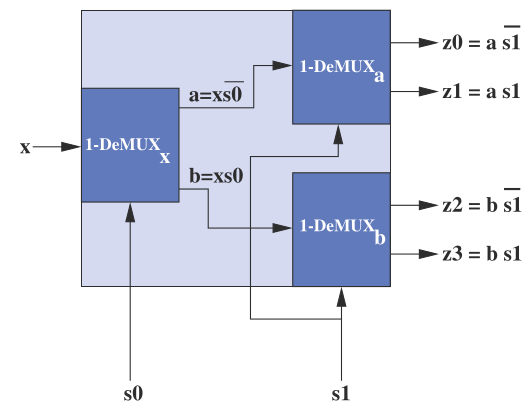
\includegraphics[scale=0.3]{pictures/2demux_td}\
\caption{1-Demultiplexer mit zugehöriger Schaltung.}
\end{figure}
\end{column}%
\end{columns}
\end{frame}

\section{Recap Normalformdarstellungen}
\begin{frame}{Recap Normalformdarstellungen}
\begin{itemize}
	\item Normalform beschreibt eine eindeutige Darstellung
	\item Vollform: Ausdruck, in dem jede Variable genau einmal vorkommt 
	\item Literal: Teilausdruck, der entweder negierte oder unnegierte Variable darstellt
	\item Wahrheitstafeldarstellung ist eine Art der Normalformdarstellungen
	\item Bool'sche Ausdrücke hingegen sind keine Normalformdarstellung
	\begin{itemize}
		\item Jede bool'sche Funktion durch unendlich viele Ausdrücke beschrieben werden
	\end{itemize}
\end{itemize}
\end{frame}

\begin{frame}{Normalformdarstellungen}
\begin{itemize}
	\item Vollform: Ausdruck, in dem jede Variable genau einmal vorkommt 
	\item Vollkonjunktion (\textbf{Minterm}): Ausdruck, in dem sämtliche vereinbarten Variablen (bzw. deren Negate) konjunktiv verbunden sind 
	\begin{itemize}
		\item Beispiel: $A,B,C: A \land \neg B \land C$
	\end{itemize}
	\item Volldisjunktion (\textbf{Maxterm}): Ausdruck, in dem sämtliche vereinbarten Variablen (bzw. deren Negate) disjunktiv verbunden sind
	\begin{itemize}
		\item Beispiel: $A,B,C: A \lor \neg B \lor \neg C$
	\end{itemize}
	\item Negationen nur in atomarer Form
	\begin{itemize}
		\item $\neg(A \land B)$: nicht atomar  
		\item $(\neg A \lor \neg B)$: atomar
	\end{itemize}
\end{itemize}
\end{frame}

\begin{frame}{Formale Definition}
\begin{definition}[Minterm, Maxterm, Literal]
Sei $f(x_1 ,\ldots , x_n)$ eine beliebige $n$-stellige boolesche Funktion. Jeder Ausdruck der Form
$$
	\hat{x_1} \land \ldots \land \hat{x_n} \text{\quad mit } \hat{x_i} \in \{\overline{x_i}, x_i\} 
$$
heißt \textbf{Minterm}, jeder Ausdruck der Form
$$
	\hat{x_1} \lor \ldots \lor \hat{x_n} \text{\quad mit } \hat{x_i} \in \{\overline{x_i}, x_i\} 
$$
wird \textbf{Maxterm} genannt.\\
Der Teilausdruck $\hat{x_i}$, der entweder aus einer negierten oder einer unnegierten Variablen besteht, heißt \textbf{Literal}.
\end{definition}
\end{frame}

\subsection{Disjunktive Normalform}
\begin{frame}{Disjunktive Normalform}
\begin{itemize}
	\item Die disjunktive Normalform (DNF) ist jene Darstellungsart, bei der eine Reihe von Vollkonjunktionen disjunktiv verknüpft wird. Negationen  treten nur in atomarer Form auf.
	\begin{itemize}
		\item $(A \land \neg B \land C) \lor (A \land B \land C) \lor (\neg A \land \neg B \land C)$ 
	\end{itemize}
	\item Andere Bezeichnungen:
	\begin{itemize}
		\item Kanonische disjunktive/konjunktive Normalform (KDNF/KKNF)
		\item Vollständige disjunktive/konjunktive Normalform
	\end{itemize}
\end{itemize}
\end{frame}

\begin{frame}{Beispiel: Disjunktive Normalform}
$f(x_1, x_2, x_3) = (x_1 \Rightarrow x_2) \land (\neg x_1 \Leftrightarrow x_3)$
\begin{table}[]
\begin{tabular}{|c|c|c|c||c|c|c|}
\hline
 & $x_1$ & $x_2$ & $x_3$ & $x_1 \Rightarrow x_2$ & \textbf{$\neg x_1 \Leftrightarrow x_3$} & \textbf{$(x_1 \Rightarrow x_2) \land (\neg x_1 \Leftrightarrow x_3)$} \\ \hline
1 & 0 & 0 & 0 & 1 & 0 & 0 \\ \hline
2 & 0 & 0 & 1 & 1 & 1 & 1 \\ \hline
3 & 0 & 1 & 0 & 1 & 0 & 0 \\ \hline
4 & 0 & 1 & 1 & 1 & 1 & 1 \\ \hline
5 & 1 & 0 & 0 & 0 & 1 & 0 \\ \hline
6 & 1 & 0 & 1 & 0 & 0 & 0 \\ \hline
7 & 1 & 1 & 0 & 1 & 1 & 1 \\ \hline
8 & 1 & 1 & 1 & 1 & 0 & 0 \\ \hline
\end{tabular}
\end{table}
Vollkonjunktion/Minterm: 2: $(\neg x_1 \land \neg x_2 \land x_3)$, 4:$(\neg x_1 \land x_2 \land x_3)$, 7:$(x_1 \land x_2 \land \neg x_3)$ \\
DNF: $(\neg x_1 \land \neg x_2 \land x_3) \lor (\neg x_1 \land x_2 \land x_3) \lor (x_1 \land x_2 \land \neg x_3)$
\end{frame}

\subsection{Konjunktive Normalform}
\begin{frame}{Konjunktive Normalform}
\begin{itemize}
	\item Die konjunktive Normalform (KNF) ist jene Darstellungsart, bei der eine Reihe von Volldisjunktionen konjunktiv verknüpft wird. Negationen treten nur in atomarer Form auf.
	\begin{itemize}
		\item $(\neg A \lor \neg B \lor \neg C) \land (A \lor B \lor C) \land (A \lor \neg B \lor \neg C)$ 
	\end{itemize}
	\item Andere Bezeichnungen:
	\begin{itemize}
		\item Kanonische disjunktive/konjunktive Normalform (KDNF/KKNF)
		\item Vollständige disjunktive/konjunktive Normalform
	\end{itemize}
\end{itemize}
\end{frame}

\begin{frame}{Beispiel: Konjunktive Normalform}
\vspace*{-0.325cm}
$f(x_1, x_2, x_3) = (x_1 \land x_2) \lor x_3$
\begin{table}[]
\scalebox{0.8}{
\begin{tabular}{|c|c|c|c||c|c|}
\hline
 & $x_1$ & $x_2$ & $x_3$ & \textbf{$x_1 \land x_2$} & \textbf{$(x_1 \land x_2) \lor x_3$} \\ \hline
1 & 0 & 0 & 0 & 0 & 0  \\ \hline
2 & 0 & 0 & 1 & 0 & 1  \\ \hline
3 & 0 & 1 & 0 & 0 & 0  \\ \hline
4 & 0 & 1 & 1 & 1 & 1  \\ \hline
5 & 1 & 0 & 0 & 0 & 0  \\ \hline
6 & 1 & 0 & 1 & 0 & 1  \\ \hline
7 & 1 & 1 & 0 & 1 & 1  \\ \hline
8 & 1 & 1 & 1 & 1 & 1 \\ \hline
\end{tabular}%
}
\end{table}
Vollkonjunktion/Minterm: 1: $\neg(\neg x_1 \land \neg x_2 \land \neg x_3)$, 3: $\neg(\neg x_1 \land x_2 \land \neg x_3)$, 5: $\neg(x_1 \land \neg x_2 \land \neg x_3)$\\
Volldisjunktion/Maxterm: 1: $(x_1 \lor x_2 \lor x_3)$, 3: $(x_1 \lor \neg x_2 \lor x_3)$, 5: $(\neg x_1 \lor x_2 \lor x_3)$\\
KNF: $(x_1 \lor x_2 \lor x_3) \land (x_1 \lor \neg x_2 \lor x_3) \land (\neg x_1 \lor x_2 \lor x_3)$
\end{frame}

\subsection{Allgemeines Verfahren beim Erstellen einer Schaltung}
\begin{frame}{Allgemeines Verfahren beim Erstellen einer Schaltung}
\begin{itemize}
	\item Zusammengefasst gilt folgendes Verfahren beim Erstellen einer Schaltung:
	\begin{enumerate}
		\item Aufstellen der Wahrheitstabelle zur gesuchten Schaltung
		\item Beim Herleiten einer Normalform zwei Möglichkeiten:
		\begin{itemize}
			\item Disjunktive Normalform: Vollkonjunktion bilden alle Zeilen denen 1 zugeordnet ist, mit 0 belegte Variablen negieren. Disjunktive Verknüpfung der Vollkonjunktionen.
			\item Konjunktive Normalform: Bilden der Volldisjunktion, Wahrheitstabelle dessen Zeilen 0 zugeordnet ist, Variablen mit 1 belegt werden negiert. Diese Volldisjunktionen werden dann konjunktiv verknüpft.
		\end{itemize}
		\item Minimierungversuch mittels Äquivalenzumformungen via booleschen Algebra.
	\end{enumerate}
\end{itemize}
\end{frame}

\section{Programmable Logic Array (PLA)}
\begin{frame}{Programmable Logic Array (PLA)}
\begin{itemize}
	\item Form der programmierbaren logischen Schaltung
	\begin{itemize}
		\item \enquote{Logisches Programmieren in Hardware}
	\end{itemize}
	\item PLA hat eine Menge von Inputs als Eingabe und zwei Stufen von Logiken
	\begin{itemize}
		\item ein Feld von ANDs
		\begin{itemize}
			\item Generiert eine Menge von Produkten (Konjunktionen)
			\item Auswahl der Konjunktionsterme durch Entfernen von Schaltgliedern (aus der UND-Matrix)
		\end{itemize}
		\item Ein Feld von ORs
		\begin{itemize}
			\item Disjunktive Verknüpfung der Konjunktionsterme erfolgt mittels der ODER-Matrix
		\end{itemize}
	\end{itemize}
	\item Da jede Schaltfunktion kann als DNF (sum of products form) oder KNF (product of sums form) dargestellt werden kann
	\begin{itemize}
		\item Ist eine Realisierung von Schaltungen mithilfe von DNF/KNF möglich
	\end{itemize}
	\item PLAs verwenden üblicherweise DNFs verwendet
\end{itemize}

\end{frame}

\begin{frame}{Schaltkreisrealisierung durch PLAs}
\begin{columns}[T] % align columns
\begin{column}{.6\textwidth}
\begin{itemize}
	\item Üblicherweise wird die DNF verwendet
	\item Ausgangsbasis Wahrheitswertetabelle, Eingabekombinationen als Produkte mit Ausgabe 1
	\item Diese Herangehensweise führt zu einer Zwei-Level-Repräsentation
	\item PLA: Halbleiterschaltkreis, bestehend aus hintereinander geschalteten AND- und OR-Matrizen, um Schaltwerke für logische Funktionen in DNF zu erstellen
\end{itemize}
\end{column}%
\hfill%
\begin{column}{.48\textwidth}
\centering
%\vspace*{-1.7cm}
\begin{figure}
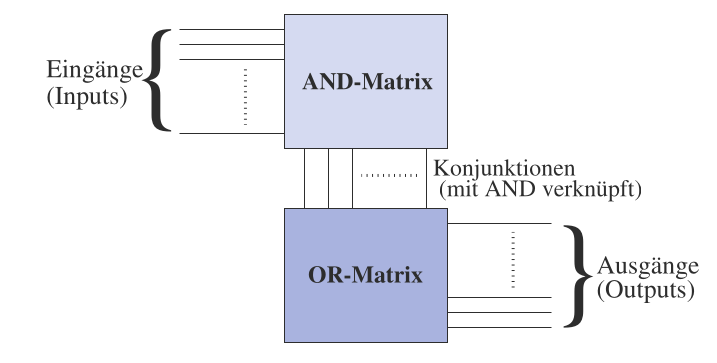
\includegraphics[scale=0.275]{pictures/pla}\
\caption{Programmable Logic Array (PLA)}
\end{figure}
\end{column}%
\end{columns}
\end{frame}

\begin{frame}{Schaltkreisrealisierung durch PLAs}
\begin{itemize}
	\item Die AND-Matrix repräsentiert dabei die Konjunktionsterme
	\begin{itemize}
		\item Termauswahl erfolgt bei der Programmierung mittels eines speziellen Geräts durch das Entfernen von Schaltgliedern aus der AND-Matrix
	\end{itemize}		
	 \item Disjunktive Verknüpfung der Konjunktionsterme erfolgt mit der OR-Matrix
\end{itemize}
\begin{center}
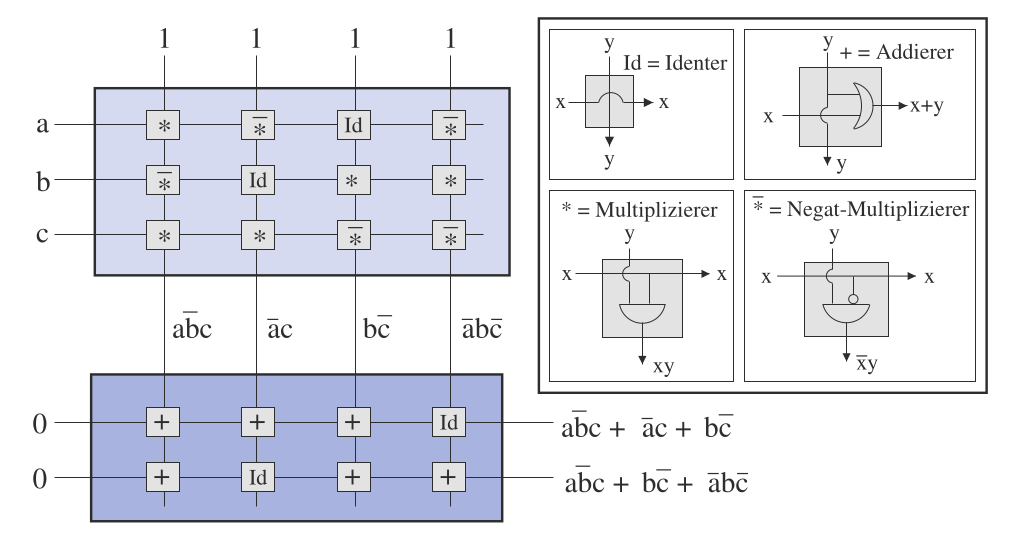
\includegraphics[scale=0.275]{pictures/pla_schaltung}
\end{center}
\end{frame}

\begin{frame}{Schaltkreisrealisierung durch PLAs}
\begin{columns}[T] % align columns
\begin{column}{.82\textwidth}
\begin{itemize}
	\item Zuordnung numerischer Wert zu Schaltungstyp: Giterpunkt via $s,t$ $\to$ Bausteintyp (eigentliche Programmierung)
	\item Überführung der Logik-Gitter in Matrix der Form: $(n + m) \times k$
	\begin{itemize}
		\item $n$ die Anzahl der Variablen,
		\item $m$ die Anzahl der verschiedenen booleschen Funktionen und
		\item $k$ die Anzahl der Teilterme ist
	\end{itemize}
	\item Ersten $n$ Zeilen dieser Matrix kommen dabei nur die Werte $0, 2$ und $3$
	\item Letzten $m$ Zeilen nur die beiden Werte $0$ und $1$
	$\begin{pmatrix}
	2 & 3 & 0 & 3 \\
	3 & 0 & 2 & 2 \\
	2 & 2 & 3 & 3 \\ \hline
	1 & 1 & 1 & 0 \\ 
	1 & 0 & 1 & 0 \\
	\end{pmatrix}$
\end{itemize}
\end{column}%
\hfill%
\begin{column}{.3\textwidth}
\centering
\hspace*{-2.7cm}
\begin{figure}
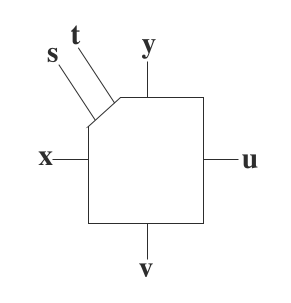
\includegraphics[scale=0.275]{pictures/pla1}\\
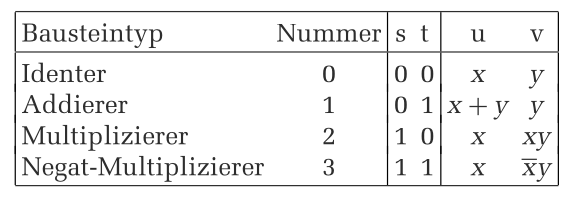
\includegraphics[scale=0.2]{pictures/pla2}
\caption{Über zwei Zuleitungen s und t programmierbarer Gitterbaustein.}
\end{figure}
\end{column}%
\end{columns}
\end{frame}

\begin{frame}{Schaltkreisrealisierung durch PLAs}
\begin{columns}[T] % align columns
\begin{column}{.7\textwidth}
\begin{itemize}
	\item Horizontal sind die Eingangssignale in die AND-Matrix
	\item Produkt-Term-Lines sind die vertikalen Eingangsignale
	\item Ausgaben sind $u, v$
	\item Folgenden Schaltfunktionen können hergeleitet werden:
	$$ u = x + \overline{s}ty ,\qquad v = \overline{s}y + sy(t \oplus x) $$
\end{itemize}
\end{column}%
\hfill%
\begin{column}{.4\textwidth}
\centering
%\vspace*{-1.7cm}
\begin{figure}
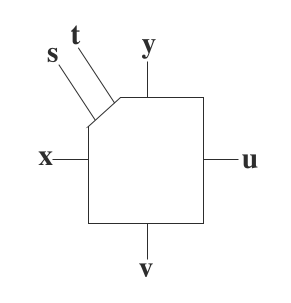
\includegraphics[scale=0.275]{pictures/pla1}\\
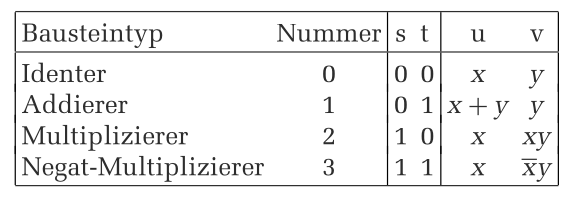
\includegraphics[scale=0.2]{pictures/pla2}
\caption{Über zwei Zuleitungen s und t programmierbarer Gitterbaustein.}
\end{figure}
\end{column}%
\end{columns}
\end{frame}

\begin{frame}{Schaltkreisrealisierung durch PLAs}
\begin{itemize}
	\item Ursprünglich wurde eine Matrix aus Sicherungen (Fuse Network) verwendet
	\begin{itemize}
		\item Programmierung: Zu realisierenden logischen Funktion, einzelne Sicherungen mittels hohen Strom durchgebrannt
		\item Problem: Über größere Zeiträume werden einzelne Sicherungen auf Grund von Kristallisierung wieder leitend 
	\end{itemize}
	\item Anti-Fuse-Technologie: Besteht PLA aus einer Diodenmatrix, jede Diode ein Bit repräsentiert
	\item Dioden so verschalten, dass sie den Strom sperren
	\begin{itemize}
		\item Programmierung:  Gezieltes zerstören bestimmter Dioden mittels eines sehr hohen Stroms 
		\item Hierdurch wird leitende Verbindung realisiert
		\item Nach dem \enquote{Brennen} werden die geschriebenen Daten durch Bitmuster defekter/funktionierender Dioden repräsentiert
	\end{itemize}
	\item Daten beliebig oft auslesbar, einmal programmierbar -- keine Änderungen
\end{itemize}
\end{frame}


\begin{frame}{Nutzung PLAs}
\begin{itemize}
	\item Lösung: GAL (Generic Array Logic)
	\item PLAs nur für kleine Logikbausteine, größere Probleme mit ASIC, FPGA und CPLD etc.
	\item Programmable Array Logic (PAL, nur AND-Matrix programmierbar) und Programmable Read-Only Memory (PROM, nur OR-Matrix programmierbar)
	\item PLA für Kontrolle von Datenpfade -- Definiert Zustände im Instruction-Set und gibt zulässige Folgezustänge vor
	\item PLAs als Zählfunktion
	\item PLA als Decoder 
	\item PLA als BUS-Schnittstelle für IO-Programmierung
\end{itemize}
\end{frame}

\begin{frame}{Plakatives Beispiel}
\begin{itemize}
	\item Eingangssignal 1:  Anschaltknopf (an/aus)
	\item Eingangssignal 2:  Sicherheitsschalter (an/aus)
	\item Ausgangssignal:    Motor (an/aus)
	\item Mögliche Programmierung: 
	\begin{itemize}
		\item Wenn Anschaltknopf = an  UND  Sicherheitsschalter = an,  dann Motor = an.
		\item Wenn Anschaltknopf = an  UND  Sicherheitsschalter = aus  ODER
		\item wenn Anschaltknopf = aus UND  Sicherheitsschalter = an   ODER
		\item wenn Anschaltknopf = aus UND  Sicherheitsschalter = aus, dann Motor = aus.
	\end{itemize}
\end{itemize}
\cite{WikiPLA}
\end{frame}



\section*{Quellen}
\appendix
\begin{frame}[allowframebreaks]
  \frametitle<presentation>{Quellen}
\printbibliography
\end{frame}
\end{document}